\section{Formulation par éléments finis --- Cas 1D}

Dans cette partie, l'objectif est d'exprimer le problème de la propagation acoustique dans une cavité unidimensionnelle
en utilisant le formalisme "éléments finis".

Le schéma du problème est présenté en figure~\ref{fig:FEM:propa_1D}.

\begin{figure}[!ht]
	\centering
	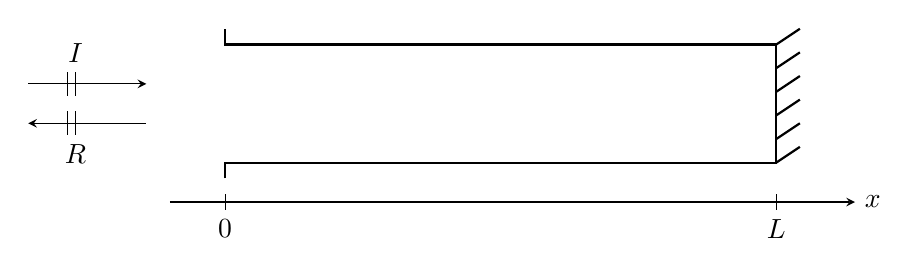
\begin{tikzpicture}[>=stealth]

	% waveguide
	\draw[thick] (0,.3) -- (0,.5) -- (7,.5) -- (7,2) -- (0,2) -- (0,2.2);
	\foreach \i in {0,...,5}{
		\draw[thick] (7,\i*0.3+0.5) -- ++(.3,.2);
	}
	
	% x axis
	\draw[->] (-.7,0) -- (8,0) node[right] {$x$};
	\draw (0,.1) -- ++(0,-.2) node[below] {$0$};
	\draw (7,.1) -- ++(0,-.2) node[below] {$L$};

	% waves
	% R
	\draw[<-] (-2.5,1) -- ++(1.5,0);
	\draw (-2,1.15) -- ++(0,-.3);
	\draw (-1.9,1.15) -- ++(0,-.3) node[below] {$R$};

	% I
	\draw[->] (-2.5,1.5) -- ++(1.5,0);
	\draw (-2,1.65) -- ++(0,-.3);
	\draw (-1.9,1.65) node[above] {$I$} -- ++(0,-.3);

\end{tikzpicture}


	\caption{\label{fig:FEM:propa_1D}Schéma du problème de propagation dans une cavité acoustique 1D de longueur L.}
\end{figure}

\subsection{Partie théorique}

\subsubsection{Formulation par éléments finis}
\label{FEM1D:subsection:linear}

\paragraph{Position du Problème}

Le domaine considéré est noté $\Omega$ et sa frontière $\partial\Omega$.

Les conditions aux limites en $x=0$ et $x=L$ imposent :

\begin{equation}
	\left\{\begin{array}{l}
	\left.\partial_np\right|_{x=L} = 0\\
	\left.p\right|_{x=0} = p_i+p_r
	\end{array}\right. \label{FEM1D:BC}
\end{equation}


\paragraph{Formulation Variationnelle}

Le problème est régi par l'équation d'Helmholtz sans source telle que présentée en~\eqref{FEM1D:helm} (avec $k =
\nicefrac{\omega}{c}$ le nombre d'onde, $c$ la célérité du son dans le milieu, et $\omega$ la pulsation).

\begin{equation}
	(\Delta + k^2)p(x,\omega) = 0 \label{FEM1D:helm}
\end{equation}

En faisant usage de la formulation variationnelle (avec $\DP$ le champ variationnel), puis d'une intégration par
parties, le problème s'exprime comme en~\eqref{FEM1D:IPP}.

\begin{eqnarray}
	\int_\Omega \Delta p~\DP~\dd\Omega + k^2 \int_\Omega p~\DP~\dd\Omega & =  & 0,\quad \forall\DP\notag\\
	\int_\Omega p''~\DP~\dd\Omega + k^2 \int_\Omega p~\DP~\dd\Omega & =  & 0,\quad \forall\DP\notag\\
	\bigg[p'~\DP\bigg]_{\partial\Omega} - \int_\Omega p'~\DP' ~\dd\Omega + k^2\int_\Omega p~\DP~\dd\Omega & = & 0, \quad \forall\DP \label{FEM1D:IPP}
\end{eqnarray}

Considérant les conditions aux limites, il est possible de simplifier le crochet comme suit.

\begin{equation}
	\bigg[p'~\DP\bigg]_{\partial\Omega} = \underbrace{p'(L)\DP(L)}_{=0~\because~\left.\partial_np\right|_{x=L}= 0} - p'(0)\DP(0) \label{FEM1D:crochet}\\
\end{equation}

En ré-injectant~\eqref{FEM1D:crochet} dans~\eqref{FEM1D:IPP} et en ré-organisant les termes, il apparait l'équation~\ref{FEM1D:pre_vect}.

\begin{equation}
	\int_\Omega p'~\DP'~\dd\Omega - k^2\int_\Omega p~\DP~\dd\Omega = -p'(0)\DP(0), \quad \forall\DP \label{FEM1D:post_IPP}
\end{equation}

\paragraph{Fonctions de forme}

Supposant que les champs $p$ et $\DP$ sur un intervale $[x_i, x_j]$ sont décomposables en une combinaison linéaire de
fonctions $\phi_k$ (dites fonctions de forme) assorties des valeurs du champs aux extrémités du domaine, il vient :

\begin{equation}
	\left\{\begin{array}{l}
		p = \phi_1(x)p(x_i) + \phi_2(x)p(x_j)\\
		p' = \phi_1'(x)p_i + \phi_2'(x)p(x_j)\\
	\end{array}\right., \quad
	\left\{\begin{array}{l}
		\DP = \phi_1(x)\DP(x_i) + \phi_2(x)\DP(x_j)\\
		\DP' = \phi_1'(x)\DP(x_i) + \phi_2'(x)\DP(x_j)\\
	\end{array}\right.\label{FEM1D:shapefun}
\end{equation}

Pour alléger les notations, on pose $\alpha_k\equiv \alpha(x_k)$ où $\alpha$ est un champ et $x_k$ un point, de même
$\phi_k\equiv\phi_k(x)$.

Dans un premier temps, les fonctions utilisés $\phi_{1,2}$ sont des fonctions linéaires présentant le profil présenté en
figure~\ref{fig:FEM:lin_shape_fun}. Les équations de ces fonctions sont données ci-après :

\begin{equation*}
	\phi_1 = 1-\frac{x}{h} \quad;\quad \phi_2 = \frac{x}{h}
\end{equation*}

\begin{figure}[!ht]
	\centering
	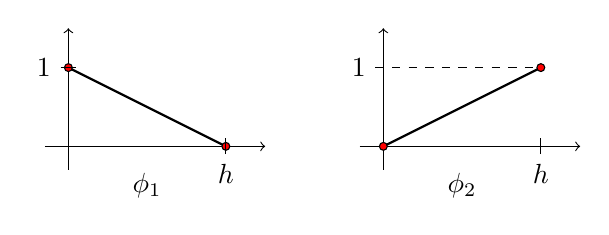
\begin{tikzpicture}
	\def\h{2};

	% PHI 1
	\draw[thick] plot [domain=0:\h] (\x,{1-\x/\h});
	\draw[->] (-.3,0) -- (\h+.5,0);
	\draw[->] (0,-.3) -- (0,1.5);
	\draw[fill=red] (0,1) circle (.05);
	\draw[fill=red] (\h,0) circle (.05);
	\draw (-.1,1) node[left] {$1$} --++(.2,0);
	\draw (\h,-.1) node[below] {$h$} --++(0,.2);
	\draw (\h*.5,-.5) node {$\phi_1$};

	% PHI 2
	\begin{scope}[shift={(\h+2,0)}]
		\draw[thick] plot [domain=0:\h] (\x,{\x/\h});
		\draw[->] (-.3,0) -- (\h+.5,0);
		\draw[->] (0,-.3) -- (0,1.5);
		\draw[fill=red] (0,0) circle (.05);
		\draw[fill=red] (\h,1) circle (.05);
		\draw[dashed] (-.1,1) node[left] {$1$} -- (\h,1);
		\draw (\h,-.1) node[below] {$h$} --++(0,.2);
		\draw (\h*.5,-.5) node {$\phi_2$};
	\end{scope}
\end{tikzpicture}


	\caption{\label{fig:FEM:lin_shape_fun}Présentation des fonctions de forme linéaires utilisées. L'élément est ici considéré
	de longueur $h$.}
\end{figure}


Il est alors possible de ré-écrire les équations de~\eqref{FEM1D:shapefun} de manière vectorielle comme présenté
en~\eqref{FEM1D:shapevec}.

\begin{equation}
	\left\{\begin{array}{l}
        p = \big[\phi_1\big|\phi_2\big]\begin{Bmatrix}p_i\\p_j\end{Bmatrix} = \big[\phi_1|\phi_2\big]\ul{p}\\
		p' = \big[\phi_1'\big|\phi_2'\big]\begin{Bmatrix}p_i\\p_j\end{Bmatrix} = \big[\phi_1'|\phi_2'\big]\ul{p}\\
	\end{array}\right.,\quad
	\left\{\begin{array}{l}
        \DP = \big[\phi_1\big|\phi_2\big]\begin{Bmatrix}\DP_i\\\DP_j\end{Bmatrix} = \big[\phi_1\big|\phi_2\big]\ul{\DP}\\
		\DP' = \big[\phi_1'\big|\phi_2'\big]\begin{Bmatrix}\DP_i\\\DP_j\end{Bmatrix} = \big[\phi_1'\big|\phi_2'\big]\ul{\DP}\\
	\end{array}\right.\label{FEM1D:shapevec}
\end{equation}

En utilisant cette dernière équation~\eqref{FEM1D:shapevec}, en considérant une partition du domaine $\Omega$ de sorte
que $\Omega = \sum_e\Omega_e$ où l'équation~\eqref{FEM1D:helm} est vérifiée sur chacune des parties de $\Omega$ et en
utilisant la relation de Chasles, il vient (de~\eqref{FEM1D:post_IPP}):

\begin{eqnarray}
	\int_\Omega p'~\DP'~\dd\Omega - k^2\int_\Omega p~\DP~\dd\Omega & = & -p'(0)\DP(0), \quad \forall\DP\notag\\
	\Leftrightarrow \sum_e \left\{\int_{\Omega_e} p_e'~\DP_e'~\dd\Omega
        - k^2\int_{\Omega_e} p_e~\DP_e~\dd\Omega \right\}
        & = & -p'(0)\DP(0), \quad \forall\DP \notag\\
	\Leftrightarrow \sum_e \bigg\{\int_{\Omega_e}
        \ul{\DP}_e^T\big[\phi_1'|\phi_2'\big]^T\big[\phi_1'|\phi_2'\big]\ul{p}_e~\dd\Omega
	   &&\notag\\
        - k^2\int_{\Omega_e}
        \ul{\DP}_e^T\big[\phi_1|\phi_2\big]^T\big[\phi_1|\phi_2\big]\ul{p}_e~\dd\Omega \bigg\}
        & = & -p'(0)\DP(0), \quad \forall\DP\notag\\
	\Leftrightarrow \sum_e \Bigg\{\int_{\Omega_e}
    \ul{\DP}_e^T\begin{bmatrix}\phi_1'^2 & \phi_1'\phi_2'\\\phi_1'\phi_2'& \phi_2'^2\end{bmatrix}\ul{p}_e~\dd\Omega
	   &&\notag\\
		   - k^2\int_{\Omega_e}
\ul{\DP}_e^T\begin{bmatrix}\phi_1^2 & \phi_1\phi_2\\\phi_1\phi_2 & \phi_2^2\end{bmatrix}\ul{p}_e~\dd\Omega \Bigg\}
        & = & -p'(0)\DP(0), \quad \forall\DP\notag\\
	\Leftrightarrow \sum_e \Bigg\{
	\ul{\DP}_e^T\underbrace{\begin{bmatrix}\int_{\Omega_e}\phi_1'^2\dd\Omega & \int_{\Omega_e}\phi_1'\phi_2'\dd\Omega\\\int_{\Omega_e}\phi_1'\phi_2'\dd\Omega& \int_{\Omega_e}\phi_2'^2\dd\Omega\end{bmatrix}}_{\uul{K}_e}\ul{p}_e
	   &&\notag\\
        - k^2
\ul{\DP}_e^T\underbrace{\begin{bmatrix}\int_{\Omega_e}\phi_1^2\dd\Omega &
\int_{\Omega_e}\phi_1\phi_2\dd\Omega\\\int_{\Omega_e}\phi_1\phi_2\dd\Omega &
\int_{\Omega_e}\phi_2^2\dd\Omega\end{bmatrix}}_{\uul{M}_e}\ul{p}_e \Bigg\}
        & = & -p'(0)\DP(0), \quad \forall\DP\notag\\
\Leftrightarrow \sum_e \left\{
        \ul{\DP}_e^T\uul{K_e}\ul{p}_e~\dd\Omega - k^2\ul{\DP}_e^T\uul{M_e}\ul{p}_e~\dd\Omega \right\}
        & = & -p'(0)\DP(0), \quad \forall\DP\label{FEM1D:elem_mat}
\end{array}
\end{equation}

Dans les équations précédentes, les quantités indicées d'un $e$ sont valables sur un élément. Les quantités soulignées
une fois sont des vecteurs, celles soulignés deux fois des matrices\footnote{Le nombre de soulignements correspondant à
l'ordre tensoriel de la quantité.}.

\paragraph{Matrices Booléennes et Vecteurs Globaux}
\newcommand{\GP}{\ul{\mathbb{P}}}
\newcommand{\GDP}{\ul{\delta\mathbb{P}}}
L'objectif est maitenant d'exprimer l'intérieur de la somme en fonction non plus des extrémités de l'éléments en cours
$\ul{p}_e$ et $\ul{\DP}_e$ mais des vecteurs globaux $\GP$ et $\GDP$.

En notant que on peut exprimer $\ul{p}_e$ sur le premier élément en fonction de $\GP$ \textit{via} :

\begin{equation*}
    \ul{p}_e =
    \underbrace{\begin{bmatrix}
         1 & 0 & 0 & \cdots & 0\\
         0 & 1 & 0 & \cdots & 0
    \end{bmatrix}}_{\uul{L}_e}\GP
\end{equation*}

De même il est possible d'exprimer $\ul{\DP}_e^T = \GDP^T\uul{L}_e^T$. En remplaçant dans~\eqref{FEM1D:elem_mat}, il
vient :

\begin{eqnarray}
    \sum_e \left\{
        \uul{\DP}_e^T\uul{K_e}\ul{p}_e~ - k^2 \ul{\DP}_e^T\uul{M_e}\ul{p}_e~ \right\}
        & = & -p'(0)\GDP_0, \quad \forall\GDP\notag\\
	\Leftrightarrow
    \sum_e \left\{
	\GDP^T\uul{L}_e^T\uul{K_e}\uul{L}_e\GP~\dd\Omega - k^2 \GDP^T\uul{L}_e^T\uul{M_e}\uul{L}_e\GP~\dd\Omega \right\}
	& = & -p'(0)\GDP_0, \quad \forall\GDP\label{FEM1D:post_boolean}
\end{eqnarray}

Comme ni $\GP$ ni $\GDP$ ne dépendent de l'élément, il est possible de les sortir de la somme, qui est ensuite
distribuée sur les deux termes comme suit :

\begin{equation*}
	\GDP^T\left[\underbrace{\sum_e \left\{ \uul{L}_e^T\uul{K_e}\uul{L}_e\right\}}_{\uul{K}}
	- k^2 \underbrace{\sum_e\left\{\uul{L}_e^T\uul{M_e}\uul{L}_e\right\}}_{\uul{M}}\right]\GP
	& = & -p'(0)\GDP_0, \quad \forall\GDP
\end{equation*}

Le fait que cette expression soit valable pour tout $\GDP$, implique :

\begin{equation}
\left[\uul{K} - k^2\uul{M}\right]\GP = \begin{Bmatrix} - p'(0) \\0\\\vdots\\0\end{Bmatrix} \label{FEM1D:final}
\end{equation}

\paragraph{Prise en compte de l'excitation}
Le problème est posé de sorte que l'entrée du résonateur est excitée par une onde plane se propageant vers les $x$
croissants et que les interactions à l'interface produisent une onde plane réfléchie se propageant vers les $x$
décroissants. Ainsi, en notant $p_i$ l'onde incidente et $p_r$ l'onde réfléchie :

\begin{equation}
	\left\{
	\begin{array}{l}
		p_i(x) = 1e^{-jk_xx}\\
		p_r(x) = Re^{+jk_xx}
	\end{array}
	\right.\label{FEM1D:expr_ondes}
\end{equation}

La continuité des pression et des vitesses normales en $x=0$ amène :

\begin{equation*}
	p(0) = e^{-jk_x\times0}+Re^{jk_x\times0} \Leftrightarrow p'(0) = jk(R-1)
\end{equation*}

En remplaçant ce dernier résultat dans~\eqref{FEM1D:final}, il vient :

\begin{equation}
\left[\uul{K} - k^2\uul{M}\right]\GP = \begin{Bmatrix} -jk(R-1)  \\0\\\vdots\\0\end{Bmatrix} \label{FEM1D:final}
\end{equation}

Il est alors intéressant de rassembler les inconnues sur la gauche de l'équation en introduisant le vecteur étendu
suivant :

\begin{equation*}
	\ul{X} = [\GP ~|~ R]^T
\end{equation*}

Il est aussi nécéssaire d'étendre la matrice de la partie gauche d'une colonne. Pour maintenir des dimensions cohérentes
dans le système d'équations, il faudra enfin retranscrire la condition de continuité suivante sur la dernière ligne :

\begin{equation*}
	\uul{P}_0 = 1 + R
\end{equation*}

\begin{equation}
	\underbrace{\left(~
	\begin{array}{cccc|c}
		&&&&jk\\
		&&&&0\\
		& & \uul{K} - k^2\uul{M} & &\vdots \\
		&&&&0\\\hline
			1 & 0 & \cdots & 0& -1 \\
	\end{array}
	~\right)}_{\uul{A}}
	\underbrace{\left\{~
	\begin{matrix}
		\\
		\\
		\GP\\
		\\\hline
		R
	\end{matrix}
	~\right\}}_{\ul{X}} = 
	\underbrace{\left\{~
	\begin{matrix}
		jk\\
		0\\
		\vdots\\
		0\\\hline
		1
	\end{matrix}
	~\right\}}_{\ul{b}}
\end{equation}

La résolution se fait alors simplement sur un système de calcul matriciel :

\begin{equation*}
	\ul{X} = \uul{A}^{-1}\ul{b}
\end{equation*}



\subsubsection{Solution Analytique}

Afin d'apprécier la qualité de l'approximation par éléments finis, il est nécessaire de disposer d'une solution
analytique. Le problème est ici posé de sorte que l'impédance en $x=L$ est connue (voir équation~\eqref{FEM1D:ana:ZL}).

\begin{equation}
	Z_L = Z(L) \rightarrow \infty \label{FEM1D:ana:ZL}
\end{equation}

En utilisant la théorie des lignes (et en particulier la formule de l'impédance ramenée), il vient (avec $Z_c =
\rho c$ l'impédance caractéristique):

\begin{eqnarray}
	Z_i = Z(0) 	& = & Z_c \frac{Z_L+jZ_c\tan(kL)}{Z_c + jZ_L\tan(kL)}\notag\\
			    & = & Z_c \frac{Z_L}{Z_L}\frac{1+j\nicefrac{Z_c}{Z_L}\tan(kL)}{\nicefrac{Z_c}{Z_L} + j\tan(kL)}\notag\\
		    Z_i & \overset{Z_L\rightarrow\infty}{\approx} & Z_c\frac{1}{j\tan(kL)}\label{FEM1D:ana:Zi}
\end{eqnarray}

En considérant une onde incidente d'amplitude 1 (en incidence normale) générant, à l'interface, une onde transmise (dans le
résonateur) et une onde réfléchie d'amplitude $R$ (voir le système d'équations~\eqref{FEM1D:expr_ondes}), puis en écrivant les
conditions de continuité, il vient :

\begin{equation*}
	R = \frac{Z_i-Z_c}{Z_i+Z_c}
\end{equation*}

En remplaçant~\eqref{FEM1D:ana:Zi} dans l'équation précédente :

\begin{equation}
	R = \frac{Z_c}{j\tan(k*L)}\label{FEM1D:ana:R}
\end{equation}

\subsubsection{Passage aux éléments quadratiques}

Dans la section~\ref{FEM1D:subsection:linear}, il était question d'interpoler les champs physiques par des fonctions
linéaires, et ce sur chacun des éléments. D'une manière générale, l'utilisation de polynôme d'ordre supérieur à 1 donne
de meilleurs résultats.

Du point de vue technique, le passage de polynômes d'ordre 1 à des polynômes d'ordre 2 passe par l'utilisation de la formule du
polynôme interpolateur de Lagrange. Le gain d'un ordre dans le polynôme est possible en ajoutant un point au centre de
l'élément. Celui-ci ne fait pas partie du maillage à proprement parler (voir figure~\ref{fig:FEM:lagrange_interp}).

\begin{figure}[!ht]
	\centering
	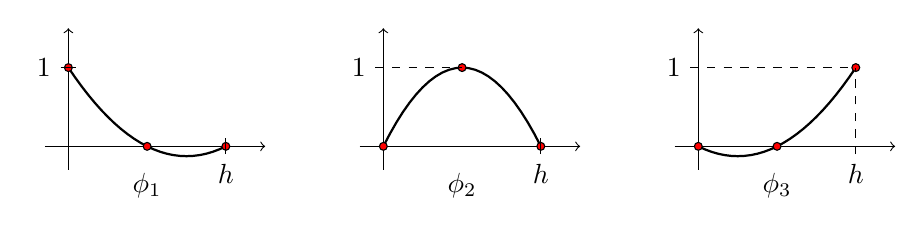
\begin{tikzpicture}
	\def\h{2};

	% PHI 1
	\draw[thick] plot [domain=0:\h] (\x,{((\h-2*\x)*(\h-\x))/(\h*\h)});
	\draw[->] (-.3,0) -- (\h+.5,0);
	\draw[->] (0,-.3) -- (0,1.5);
	\draw[fill=red] (0,1) circle (.05);
	\draw[fill=red] (\h*.5,0) circle (.05);
	\draw[fill=red] (\h,0) circle (.05);
	\draw (-.1,1) node[left] {$1$} --++(.2,0);
	\draw (\h,-.1) node[below] {$h$} --++(0,.2);
	\draw (\h*.5,-.5) node {$\phi_1$};

	% PHI 2
	\begin{scope}[shift={(\h+2,0)}]
		\draw[thick] plot [domain=0:\h] (\x,{(-4*\x*(\x-\h))/(\h*\h)});
		\draw[->] (-.3,0) -- (\h+.5,0);
		\draw[->] (0,-.3) -- (0,1.5);
		\draw[fill=red] (0,0) circle (.05);
		\draw[fill=red] (\h*.5,1) circle (.05);
		\draw[fill=red] (\h,0) circle (.05);
		\draw[dashed] (-.1,1) node[left] {$1$} -- (\h*.5,1);
		\draw (\h,-.1) node[below] {$h$} --++(0,.2);
		\draw (\h*.5,-.5) node {$\phi_2$};
	\end{scope}

	% PHI 2
	\begin{scope}[shift={({2*(\h+2)},0)}]
		\draw[thick] plot [domain=0:\h] (\x,{(\x*(2*\x-\h))/(\h*\h)});
		\draw[->] (-.3,0) -- (\h+.5,0);
		\draw[->] (0,-.3) -- (0,1.5);
		\draw[fill=red] (0,0) circle (.05);
		\draw[fill=red] (\h*.5,0) circle (.05);
		\draw[fill=red] (\h,1) circle (.05);
		\draw[dashed] (-.1,1) node[left] {$1$} -- (\h,1);
		\draw[dashed] (\h,-.1) node[below] {$h$} -- (\h,1);
		\draw (\h*.5,-.5) node {$\phi_3$};
	\end{scope}
\end{tikzpicture}

	\caption{\label{fig:FEM:lagrange_interp}Présentation des fonctions de forme utilisées. L'élément est ici considéré
	de longueur $h$.}
\end{figure}

De cette manière, les polynômes utilisés sont les suivants :

\begin{equation*}
	\phi_1 = \frac{(h-2x)(h-x)}{h^2} \quad,\quad \phi_2 = \frac{-4x(x-h)}{h^2} \quad,\quad \phi_3 = \frac{x(2x-h)}{h^2}
\end{equation*}

Dans le reste des calculs, le passage aux éléments quadratiques agrandit les matrices élémentaires (de $2\times2$ à
$3\times3$), les calculs desdites matrices sont alors réalisés par intégration numérique\footnote{Ici, en utilisant la
quadrature de Gauss et 4 points.}. Par extension, ce changement d'ordre fait aussi varier la taille de la matrice
$\uul{A} = \uul{K} - k^2\uul{M}$ qui passe de $(N+1)^2$ valeurs\footnote{Rappel : $\uul{A}$ est carrée.} à $(2N+1)^2$
valeurs. Les vecteurs $\ul{X}$ et $\ul{b}$ sont aussi adaptés en fonction de la nouvelle taille du
système.

\subsection{Simulation}

L'équation~\eqref{FEM1D:final} est facilement implémentable dans un système de calcul matriciel (ici, GNU/Octave et plus
rarement \matlab sont utilisés).

La suite compare la phase du coefficient de réflexion analytique et celle du coefficient calculé par éléments
finis.

Les résultats sont présentés en figure~\ref{fig:FEM1D:simuls}.

\begin{figure}[!ht]
	\centering
	\begin{subfigure}{0.48\textwidth}
		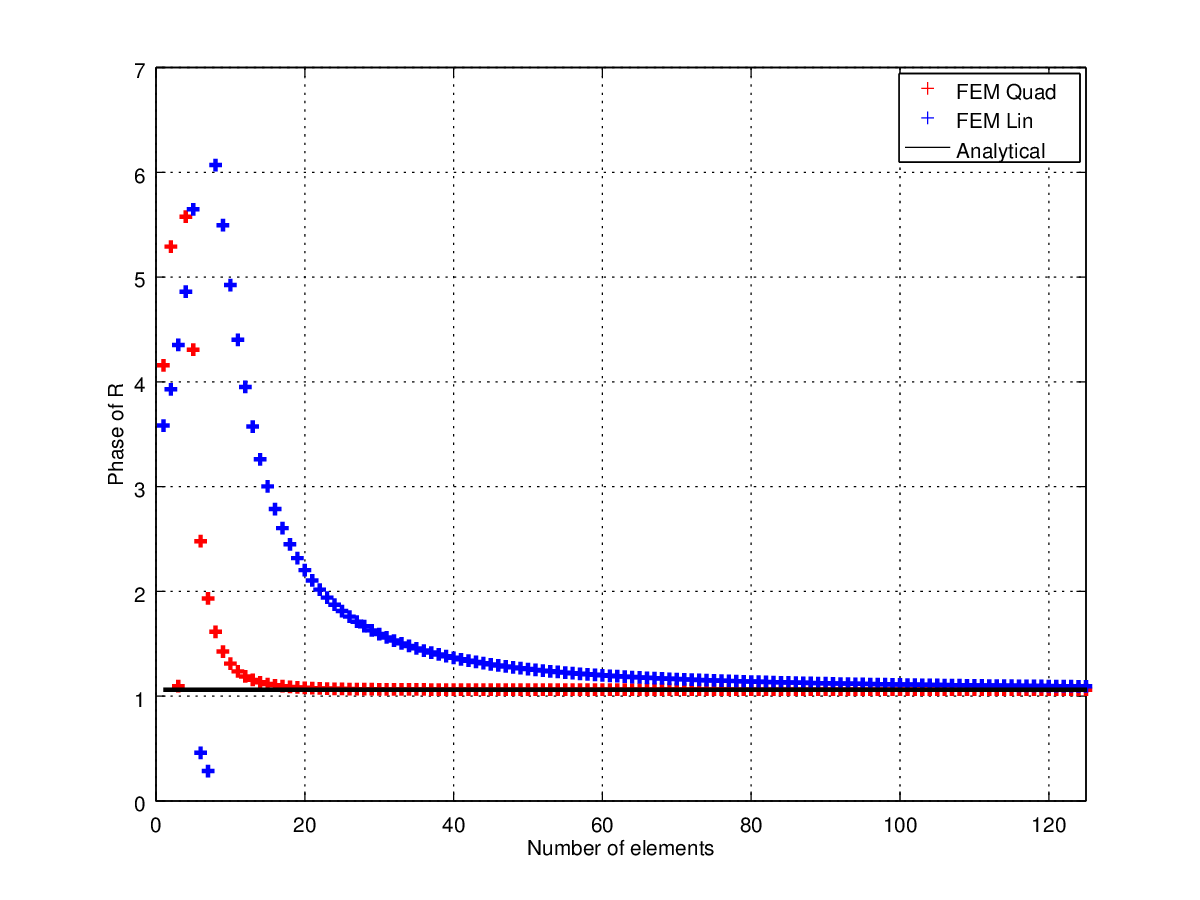
\includegraphics[width=\textwidth]{figs/FEM/simuls_1D/phase.png}
		\caption{\label{fig:FEM1D:simuls:phase}Point 1}
	\end{subfigure}~%
	\begin{subfigure}{0.48\textwidth}
		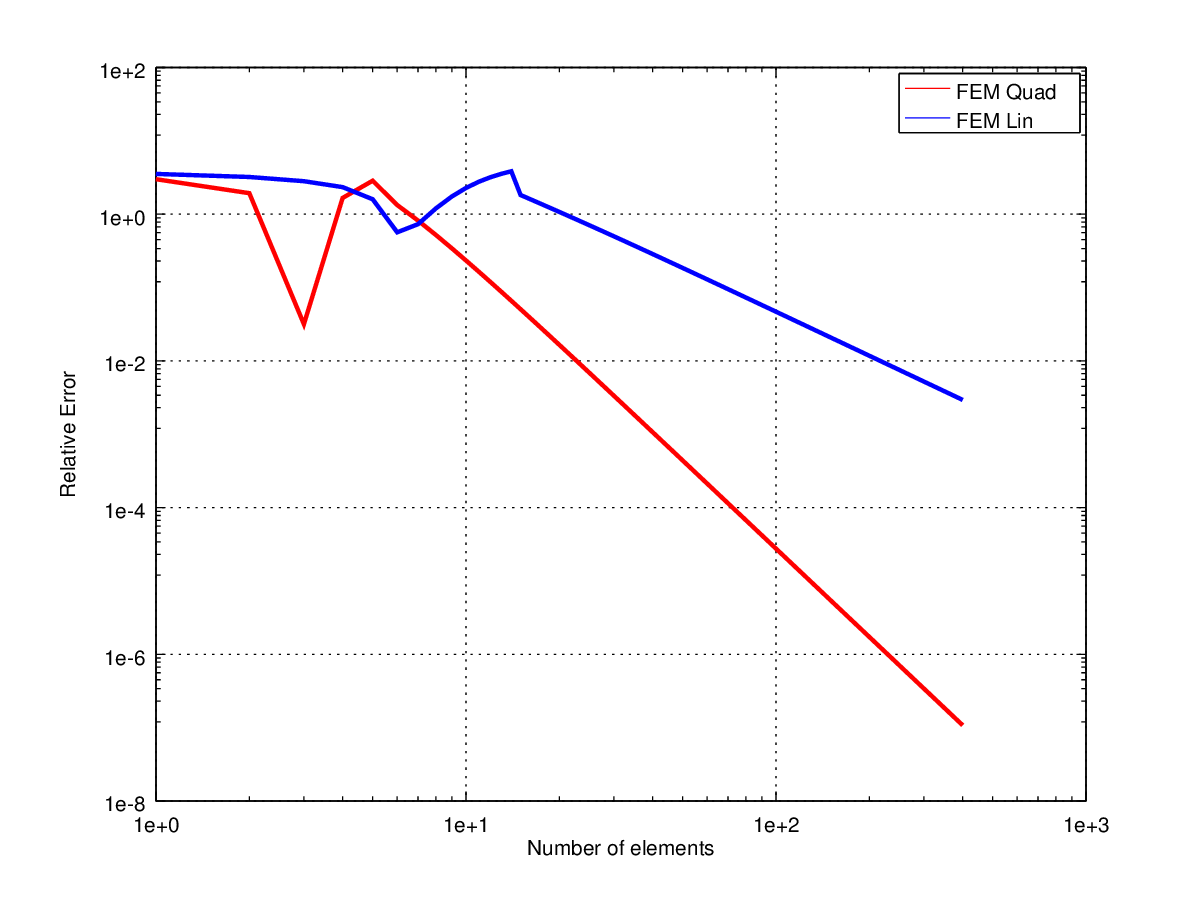
\includegraphics[width=\textwidth]{figs/FEM/simuls_1D/convergence.png}
		\caption{\label{fig:FEM1D:simuls:convergence}Point 2}
	\end{subfigure}
	\caption{\label{fig:FEM1D:simuls}Résultat des simulations. En rouge, les résultats pour des éléments quadratiques en bleu pour des éléments
	linéaires : on remarque une meilleure convergence des premiers (voir figure~\ref{fig:FEM1D:simuls:convergence}). Dans
	les deux cas, la valeur théorique est correctement approchée si l'on augmente le nombre d'éléments.}
\end{figure}

Le passage d'éléments linéaires à des éléments quadratiques augmente d'un ordre la convergence de la méthode, comme le
montre le diagramme de convergence (figure~\ref{fig:FEM:simuls:convergence}).

Il faut noter toutefois que dans un cas comme dans l'autre, l'approximation tend vers la solution exacte en augmentant
le nombre d'éléments.

Une autre limite apparaît lorsqu'est considèrée l'influence de la fréquence : en effet, pour une bonne précision de
l'approximation, il est nécessaire de disposer d'au moins 2 éléments par longueur d'onde : les méthodes par éléments
finis sont donc très gourmandes aux hautes fréquences de part la nécessité de disposer d'un maillage toujours plus fin
et donc d'augmenter drastiquement la taille des structures de donnée.
